\chapter{Transport Phenomena in Semiconductor-Superconductor Hybrid Structures}

The non-equilibrium Green's function (NEGF) technique has emerged as a powerful tool for modelling nanoscale devices. Due to the versatility of the NEGF formalism, it can also be employed for devices that incorporate superconducting elements, which are of great academic interest, especially ones involving topological superconductivity and Majorana bound states. Refer to Appendix~\ref{appendix:NEGF} for a brief discussion of the NEGF formalism used throughout the text. \par 

\section{The Bogoliubov deGennes Hamiltonian}

The {\bf B}ardeen-{\bf C}ooper-{\bf S}chreiffer theory was presented in 1956 as a variational mean-field approach to phonon-mediated inter-electron attractive interactions, leading to the formation of Cooper pairs below a critical temperature. As a superconductor is cooled below its critical temperature, the attractive interactions between electrons dominate over the repulsive Coulombic forces. In the presence of a net-attractive interaction, no matter how weak, the normal metal state becomes unstable. An attractive matrix element can arise by the coupling of electrons to another system of particles or excitations in the solid. The BCS theory was the first microscopic description of the ground state of the superconductor, following which Bogoliubov formulated a concise framework in terms of quasiparticles to describe setups which feature superconductors coupled with normal systems. \par 

A system of interacting electrons is described by the second quantization Hamiltonian, in terms of electron creation (annihilation) field operators $\Psi^{\dagger}(\textbf{r}\sigma)$ ($\Psi(\textbf{r}\sigma)$), at position $\textbf{r}$, with spin $\sigma$

\begin{equation}
        \begin{aligned}
        H &= \underbrace{H_{0}}_{\text{single-particle Hamiltonian}} +\underbrace{H_{int}}_{\text{four-fermion interaction Hamiltonian}} \\
        H_{0} &= \int d\textbf{r} \sum_{\sigma} \Psi^{\dagger}(\textbf{r}\sigma) \left[ \frac{(-i\hbar \nabla - e \textbf{A})^{2}}{2m^{*}} + U_{0}(\textbf{r}\sigma) - \mu \right] \Psi(\textbf{r}\sigma) \\
        H_{int} &= -\frac{1}{2}V \int d\textbf{r} \sum_{\sigma, \sigma'} \Psi^{\dagger}(\textbf{r}\sigma) \Psi^{\dagger}(\textbf{r}\sigma') \Psi(\textbf{r}\sigma') \Psi(\textbf{r}\sigma)
        \end{aligned}
\end{equation}
 
where $\textbf{A}$ is the magnetic vector potential, $m^{*}$ is the electron effective mass, $U_{0}$ is the single-particle potential energy and $V$ scales the interaction energy. Using the mean-field approximation, the four-fermion interaction potential can be expressed as an average potential acting on one particle at a time, which restricts the Hamiltonian to terms quadratic in field operators.

\begin{equation*}
        H_{mf} = \int d\textbf{r} \sum_{\sigma}\Psi^{\dagger}(\textbf{r}\sigma)[H_{0}+U_{\sigma}]\Psi(\textbf{r}\sigma) + \int d\textbf{r} \: [\Delta \: \Psi^{\dagger}_{\uparrow} \Psi^{\dagger}_{\downarrow} + \Delta^{*} \: \Psi_{\downarrow} \Psi_{\uparrow}]
\end{equation*}

The superconducting order parameter ($\Delta$), which couples electrons and holes of opposite spin and momentum, is the physical quantity that sets apart superconductors from a normal insulator. Apart from the conventional terms involving Coulomb interaction, which are of the form $\langle \psi_{i}^{\dagger}\psi_{j} \rangle$ (where $i$, $j$ are labelling indices for a combination of quantum-state and spin), there are anomalous terms of the form $\langle \psi_{i}^{\dagger}\psi_{j}^{\dagger} \rangle$ arising from the Cooper pairing process below the critical temperature. \par 

As per the BCS theory, the indices can be transformed as $i \rightarrow k \uparrow$, and $j \rightarrow -k \downarrow$ for a continuum model. Assuming a metallic system, we end up with up-spin and down-spin bands filled up to the Fermi level designated by the electrochemical potential $\mu$. A ``hole'' transformation can be performed on the down-spin band, which flips the band, and the down-spins are now represented by unfilled particles or holes, similar to semiconductor physics. This is equivalent to a 2-component spinor transformation:

\begin{equation}
    \begin{bmatrix}
        \Psi^{\dagger}_{\uparrow}(\textbf{r}) \\
        \Psi^{\dagger}_{\downarrow}(\textbf{r})
     \end{bmatrix} \rightarrow
     \begin{bmatrix}
        \Psi^{\dagger}_{\uparrow}(\textbf{r})\\
        \Psi_{\downarrow}(\textbf{r})
     \end{bmatrix} (\text{in real space}), \: 
     \begin{bmatrix}
        c^{\dagger}_{k \uparrow} \\
        c^{\dagger}_{-k \downarrow}    
     \end{bmatrix} \rightarrow
     \begin{bmatrix}
        c^{\dagger}_{k\uparrow} \\
        c_{-k\downarrow}   
     \end{bmatrix} (\text{in \textit{k}-space})
\end{equation}

The Hamiltonian of the continuum model is a $2 \times 2$ matrix in $k$-space, with two dispersion relations that get coupled due to the pairing term $\Delta_{k}$.

\begin{equation*}
    H_{k} = \begin{bmatrix}
            (\epsilon_{k}-\mu) & \Delta_{k} \\
            \Delta^{*}_{k} & -(\epsilon_{k}-\mu)
    \end{bmatrix}
\end{equation*}

where, $\epsilon_{k} = \frac{\hbar^{2}k^{2}}{2m^{*}}$. \par 

We can discretise the continuum model described above into a lattice model with a spacing of $a$. The on-site component of the Hamiltonian is given as 

\begin{equation}
    \alpha_{S} = \begin{bmatrix}
          2t-\mu & \Delta_{0} \\
          \Delta_{0}^{*} & -(2t-\mu)  
    \end{bmatrix}
\end{equation}

where, $t = \frac{\hbar^{2}}{2m^{*}a^{2}}$ is the nearest-neighbour hopping parameter. The nearest-neighbour hopping matrix is given by 

\begin{equation}
    \beta = \begin{bmatrix}
          -t & 0\\
          0 & t  
    \end{bmatrix}    
\end{equation}

The tight-binding Hamiltonian is subsequently written as

\begin{equation}
    H = \sum_{i}^{N}c^{\dagger}_{i}\alpha_{S}c^{i} + \sum_{i\neq j}^{N}c^{\dagger}_{i}\beta c_{j}    
\end{equation}

where $c^{\dagger}_{i}$ is the creation operator of the Nambu 2-component spinor ar site $i$, and $N$ is the number of sites in the device. The Hamiltonian of the superconducting sample can be written in the general form 

\begin{equation}
H = \begin{pmatrix}
\alpha_S & \beta & 0 & \dots & 0 \\
\beta^{\dagger} & \alpha_S & \beta & 0 & 0 \\
0 & \beta^{\dagger} & \alpha_S & \beta & \vdots \\
\vdots & 0 & \ddots & \ddots & \beta \\
0 & \dots & \dots & \beta^{\dagger} & \alpha_S \\
\end{pmatrix}   
\end{equation}


\section{The Isolated Kitaev Chain}

The field of topological superconductivity began with a lattice model proposed by Kitaev in 2001. The Kitaev chain is a tight-binding chain of $N$ lattice sites, with one spinless fermionic orbital at each site and nearest-neighbour $p$-wave superconducting pairing. The $p$-wave nature of the superconductivity couples particles of equal spin, allowing a spinless treatment. The pairing is treated in the usual mean-field approach, yielding the Kitaev grandcanonical Hamiltonian

\begin{equation}
    \hat{H}_{\text{KC}} = -\mu \sum_{j=1}^{N}c^{\dagger}_{j}c_{j} - t\sum_{j=1}^{N-1}(c^{\dagger}_{j+1}c_{j}+c^{\dagger}_{j}c_{j+1})-\Delta \sum_{j=1}^{N-1}(c^{\dagger}_{j}c^{\dagger}_{j+1}+c_{j+1}c_{j})    
\end{equation}

in terms of the fermionic creation (annihilation) field operators $c^{\dagger}_{j}$ ($c_{j}$). The hopping amplitude $t$ and the superconducting pairing constant $\Delta$ are assumed to be real quantities in this case. The chemical potential $\mu$ represents the on-site energy and can be modulated by applying a gate voltage. \par 

The Kiteav Hamiltonian has been of particular interest in the context of topological superconductivity due to the possibility of hosting Majorana zero modes (MZMs) at its end in a particular parameter range. This can be seen by expressing the Hamiltonian in terms of so-called Majorana operators $\gamma^{A,B}$,

\begin{equation}
    \begin{pmatrix}
        c_{j} \\
        c^{\dagger}_{j}    
    \end{pmatrix} = \frac{1}{\sqrt{2}}
    \begin{pmatrix}
        \gamma^{A}_{j} \\
        \gamma^{B}_{j}    
    \end{pmatrix}, \: (\gamma^{A,B})^{\dagger} = \gamma^{A,B},
\end{equation}

yielding the form

\begin{equation} \label{eq:majorana}
    \hat{H}_{\text{KC}} = -i\mu \sum_{j=1}^{N}\gamma^{A}_{j}\gamma^{B}_{j} + i(\Delta+t)\sum_{j=1}^{N-1}\gamma^{B}_{j}\gamma^{A}_{j+1}+i(\Delta-t)\sum_{j=1}^{N-1}\gamma^{A}_{j}\gamma^{B}_{j+1}  
\end{equation}

For the particular parameter settings $\Delta = \pm t$ and $\mu = 0$, which we call the Kitaev points, equation (\ref{eq:majorana}) leads to a `missing' fermionic quasiparticle $q_{\pm}$ at the extrema of the Kitaev chain:

\begin{equation}
    \begin{aligned}
       q_{+} &= \frac{1}{\sqrt{2}}(\gamma^{A}_{1}+i\gamma^{B}_{N}) \quad [\Delta = t] \\
       q_{-} &= \frac{1}{\sqrt{2}}(\gamma^{B}_{1}+i\gamma^{A}_{N}) \quad [\Delta = -t]          
    \end{aligned}    
\end{equation}

This quasiparticle has zero energy and is composed of two isolated Majorana states localised at the ends of the chain. In general, the condition of hosting MZM is not restricted to the Kitaev points. \par

\subsection{Bulk spectrum}

The Kitaev Hamiltonian in the limit of $N \rightarrow \infty$ reads in $k$-space 

\begin{equation*}
    \hat{H}_{\text{KC}} = \frac{1}{2}\sum_{k}\hat{\psi}^{\dagger}_{k}H(k)\hat{\psi}_{k}, \quad \hat{\psi}^{\dagger}_{k} = \begin{pmatrix}
       c_{k} & c_{-k}^{\dagger}     
    \end{pmatrix}^{\text{T}}     
\end{equation*}

The $2 \times 2$ BdG matrix

\begin{equation}
    H(k) = 
    \begin{bmatrix}
       -\mu-2t\:\text{cos}(ka) & -2i\Delta \: \text{sin}(ka) \\
       2i\Delta \: \text{sin}(ka) & \mu+2t\: \text{cos}(ka)         
    \end{bmatrix}    
\end{equation}

can be diagonalized to yield the excitation spectrum

\begin{equation}
    E_{\pm}(k) = \pm \sqrt{4\Delta^{2}\:\text{sin}^{2}(ka)+[\mu+2t\: \text{cos}(ka)]^{2}}    
\end{equation}

\subsection{Energy spectrum of the finite Kitaev chain}

Next, consider a finite Kitaev chain with $N$ sites and open boundary conditions, yielding $N$ allowed $k$ values. The BdG Hamiltonian of the open Kitaev chain can be expressed in the basis of standard fermionic operators $\hat{\psi} = (c_{1},\dots,c_{N},c_{1}^{\dagger},\dots,c_{N}^{\dagger})$,

\begin{equation*}
    \hat{H}_{\text{KC}} = \frac{1}{2}\hat{\psi}^{\dagger}H_{\text{KC}}\hat{\psi}     
 \end{equation*}

 where the BdG Hamiltonian $H_{\text{KC}}$ is

 \begin{equation}
     H_{\text{KC}} = \begin{bmatrix}
          C & S \\
          S^{\dagger} & -C   
     \end{bmatrix}     
 \end{equation} 

 These matrices have the tridiagonal structure

\begin{equation}
    \begin{aligned}
        C &= 
        \begin{bmatrix}
        -\mu & -t &  &  &  &  &  \\
        -t & -\mu & -t &  &  &  &  \\
         & -t & -\mu & -t &  &  &  \\
         &  & \ddots & \ddots & \ddots &  &  \\
         &  &  & -t & -\mu & -t &  \\
         &  &  &  & -t & -\mu & -t \\
         &  &  &  &  & -t & -\mu \\
        \end{bmatrix}_{N \times N} \\
        S &= 
        \begin{bmatrix}
        0 & \Delta &  &  &  &  &  \\
        -\Delta & 0 & \Delta &  &  &  &  \\
         & -\Delta & 0 & \Delta &  &  &  \\
         &  & \ddots & \ddots & \ddots &  &  \\
         &  &  & -\Delta & 0 & \Delta &  \\
         &  &  &  & -\Delta & 0 & \Delta \\
         &  &  &  &  & -\Delta & 0 \\              
        \end{bmatrix}_{N \times N}      
    \end{aligned} 
\end{equation}

the spectrum can be obtained by diagonalising $H_{\text{KC}}$ in real space. The fermionic operators associated with the Kitaev chain can be represented in several bases, each suited to facilitate some specific calculation. The default basis can be rearranged to a site-ordered particle-hole basis where $\hat{\psi} = (c_{1}^{\dagger},c_{1},\dots,c_{N}^{\dagger})$ with the BdG Hamiltonian matrix given by 

\begin{equation}
    H_{\text{KC}} = 
    \begin{bmatrix}
        \alpha & \beta &  &  &  &  &  \\
        \beta^{\dagger} & \alpha & \beta &  &  &  &  \\
        & \beta^{\dagger} & \alpha & \beta &  &  &  \\
        &  & \ddots & \ddots & \ddots &  &  \\
        &  &  & \beta^{\dagger} & \alpha & \beta &  \\
        &  &  &  & \beta^{\dagger} & \alpha & \beta \\
        &  &  &  &  & \beta^{\dagger} & \alpha \\        
    \end{bmatrix}_{N \times N}   
\end{equation}

where 

\begin{equation}
    \begin{aligned}
        \alpha &= 
        \begin{bmatrix}
            -\mu & 0 \\
            0 & \mu            
        \end{bmatrix}, \\
        \beta &= 
        \begin{bmatrix}
            -t & \Delta \\
            -\Delta & t             
        \end{bmatrix}        
    \end{aligned}    
\end{equation}

\clearpage

\vspace*{1cm}

\begin{figure}[h]
\centering
\includegraphics[scale=0.55]{KC.png}
\caption{\textit{Eigenspectrum of the finite Kitaev chain as a function of $\mu/\Delta$ for N = 25, $\Delta/t = 1.0$. Note the zero energy modes observed within the topological regime, i.e., $|\mu| < 2|t|$.}}
\end{figure}

\vspace{1cm}

We can also construct a ``disordered'' system with local inhomogeneity in the on-site potential. Such an inhomogeneity might occur due to Fermi energy mismatch as well as charge inhomogeneities in the system. For the disordered chain, the zero energy modes are observed both in the topological regime and in the trivial regime, which can make it difficult to identify genuine topological transitions in an experimental scenario.

\clearpage

\vspace*{2cm}

\begin{figure}[!htbp]
\centering
\includegraphics[scale=0.4]{KC_pristine_spectrum_21.png}
\caption{\textit{Eigenspectrum for a pristine setup with $N = 21$ and $t/\Delta = 4.1$}}
\vspace{1cm}
\includegraphics[scale=0.4]{KC_disorder_spectrum_21.png}
\caption{\textit{Eigenspectrum for a disordered setup with $N = 21$ and $t/\Delta = 4.1$}}
\end{figure}    

\clearpage

\vspace*{2cm}

\begin{figure}[!htbp]
\centering
\includegraphics[scale=0.4]{KC_pristine_spectrum_100.png}
\caption{\textit{Eigenspectrum for a pristine setup with $N = 100$ and $t/\Delta = 4.1$}}
\vspace{1cm}
\includegraphics[scale=0.4]{KC_disorder_spectrum_100.png}
\caption{\textit{Eigenspectrum for a disordered setup with $N = 100$ and $t/\Delta = 4.1$}}
\end{figure} 

\clearpage


\section{Voltage Driven Transport}

Andreev processes are fundamental to our understanding of transport phenomena across superconducting hybrid devices. They involve the reflection of an electron (hole) as a spin-reversed hole (electron), resulting in the transfer of a Cooper pair in the superconductor. Andreev reflections arise naturally from the BdG Hamiltonian, which has the form as shown in equation (\ref{eq:BdG}), and are thus characteristic processes of an N/S interface and are absent in normal junctions.

\begin{equation} \label{eq:BdG}
    H_{\text{BdG}} = \begin{bmatrix}
            H_{\uparrow}+U-\mu & \Delta \\
            \Delta^{*} & -(H_{\downarrow}+U-\mu)
    \end{bmatrix}    
\end{equation}

where $H_{\uparrow(\downarrow)}$ refers to the Hamiltonian of the up- (down)-spin sector, and $U$ refers to the local potentials that give rise to various reflection and transmission processes. The order parameter $\Delta$ can be viewed as a potential which couples the up-spin (upper) block with the down-spin (lower) block and is responsible for Andreev processes. 

\vspace{1cm}

\begin{figure}[h]
\centering
\includegraphics[scale=0.85]{andreev_reflection.png}
\caption{\textit{Andreev Reflection -- An incoming electron from the normal region is reflected as a spin-reversed hole, resulting in the transfer of a Cooper pair into the superconductor.}}
\end{figure}

\vspace{1cm}

Therefore, in superconducting systems, we end up with two distinct processes -- normal reflections, wherein electrons and holes reflect independently, and Andreev reflections, where electrons (holes) can reflect off as spin-reversed holes (electrons). 

\clearpage 

\subsection{N/S Junctions} \label{subsec:NS}

In the ballistic regime, we are familiar with the conductance quantisation in normal insulators, where each mode conducts with a conductance $G = \frac{2e^{2}}{h}$. However, as a consequence of Andreev processes, the conductance quantum is doubled in an N/S interface in the so-called ``sub-gap'' regime. Similar to the regular barrier potential in normal devices, which serve as a gap for the transmission of electrons/holes, the order parameter $\Delta$ can be thought of as a barrier in the superconducting region, which implies that the energy range $-\Delta < E < \Delta$ is unique to Andreev processes. \par 

In the electron-hole Nambu space, each contact has two components: the electron and the hole blocks. Assuming that a bias voltage $V$ is impressed on the N-side while the S-side is kept grounded, the electronic electrochemical potential translates to $\mu_{\text{N}e} = +eV$, and the hole electrochemical potential translates to $\mu_{\text{N}h} = -eV$. In layman's terms, it is as if the contact splits into two viable contacts simply as a result of the BdG framework being used to describe the junction. \par 

This can also be explained in more mathematical detail via the NEGF framework. The contact broadening matrices can be written with a general diagonal structure (due to diagonal structure of normal contacts in the Nambu space) as $\Gamma_{\alpha} = \Gamma_{\alpha}^{ee} + \Gamma_{\alpha}^{hh}$, where the superscripts $ee \: (hh)$denote the electron (hole) diagonal component of the broadening matrix, and $\alpha = \text{L/R}\/\text{N/S}$. The current across the N/S junction can be derived from the electron or hole current at the N-contact as,

\begin{equation} \label{eq:NS}
   \begin{aligned}
       I^{e(h)}_{N}(E) &= \frac{e}{h}\left(\underbrace{\textbf{Tr}(\Gamma_{L}^{ee(hh)}G^{r}\Gamma_{R}^{ee(hh)}G^{a})}_{T_{D}}\:[f_{N}^{ee(hh)}(E)-f_{S}^{ee(hh)}(E)]\right)  \\
       &+ \frac{e}{h}\left(\underbrace{\textbf{Tr}(\Gamma_{L}^{ee(hh)}G^{r}\Gamma_{L}^{hh(ee)}G^{a})}_{T_{A}}\:[f_{N}^{ee(hh)}(E)-f_{N}^{hh(ee)}(E)]\right)         
   \end{aligned}       
\end{equation}  

where the first term represents the direct transmission process of electron (hole), the second term represents the direct Andreev transmission, and the Fermi distributions are denoted by $f^{ee}_{\alpha}=f(E-\mu_{\alpha})$, $f^{hh}_{\alpha}=f(E+\mu_{\alpha})$. \par 

Given the fact that the total current (electron + hole) is double that of each sector as defined in equation (\ref{eq:NS}), the current at the N-side can be expressed in a more concise form as,

\begin{equation}
    I_{N} = \frac{2e}{h}\int dE\:(T_{D}(E)\:[f(E-eV)-f(E)]+T_{A}(E)\:[f(E-eV)-f(E+eV)])    
\end{equation}

From the above equation, one can analytically evaluate the current by setting the temperature $T \rightarrow 0$, and taking derivatives w.r.t. the applied bias at the N-side. In the sub-gap regime, Andreev transmission dominates with a probability of unity since the superconducting segment is infinitely long. From this, we get $G(V) = \frac{\partial I_{N}}{\partial V} = \frac{4e^{2}}{h}$, elucidating the conductance doubling in the sub-gap regime. In the supra-gap regime, Andreev transmission occurs alongside direct transmission, which gives a conductance $G(V) = \frac{4e^{2}}{h}T_{A} + \frac{2e^{2}}{h}T_{D}$, with a suppression of $T_{A}$ with increasing bias voltage. In the asymptotic range of large energies, only the direct transmission dominates due to the quasiparticle transmission and this leads to a conductance of $\frac{2e^{2}}{h}$ at large bias. \par 

\vspace{3cm}

\begin{figure}[h]
\centering
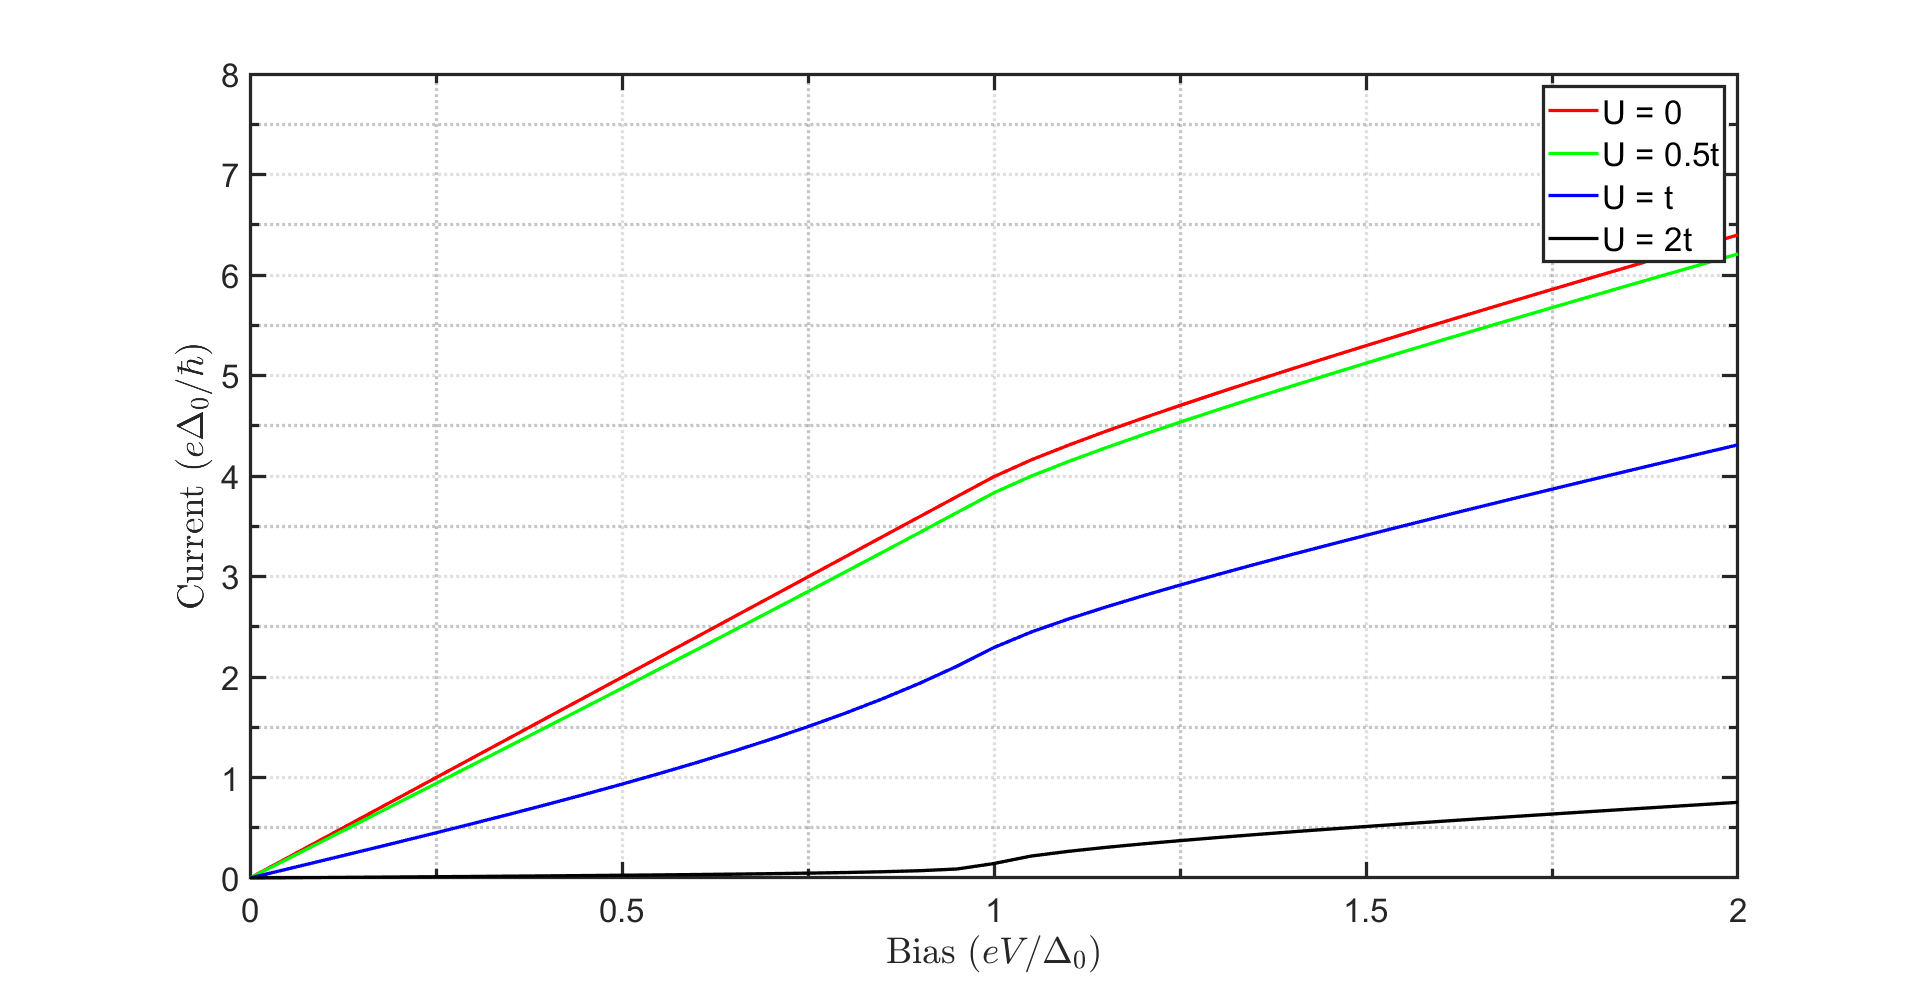
\includegraphics[scale=0.3]{I-V.png}
\caption{\textit{Current as a function of the applied bias across an N/S junction.}}
\end{figure}

\clearpage

\begin{figure}[h]
\centering
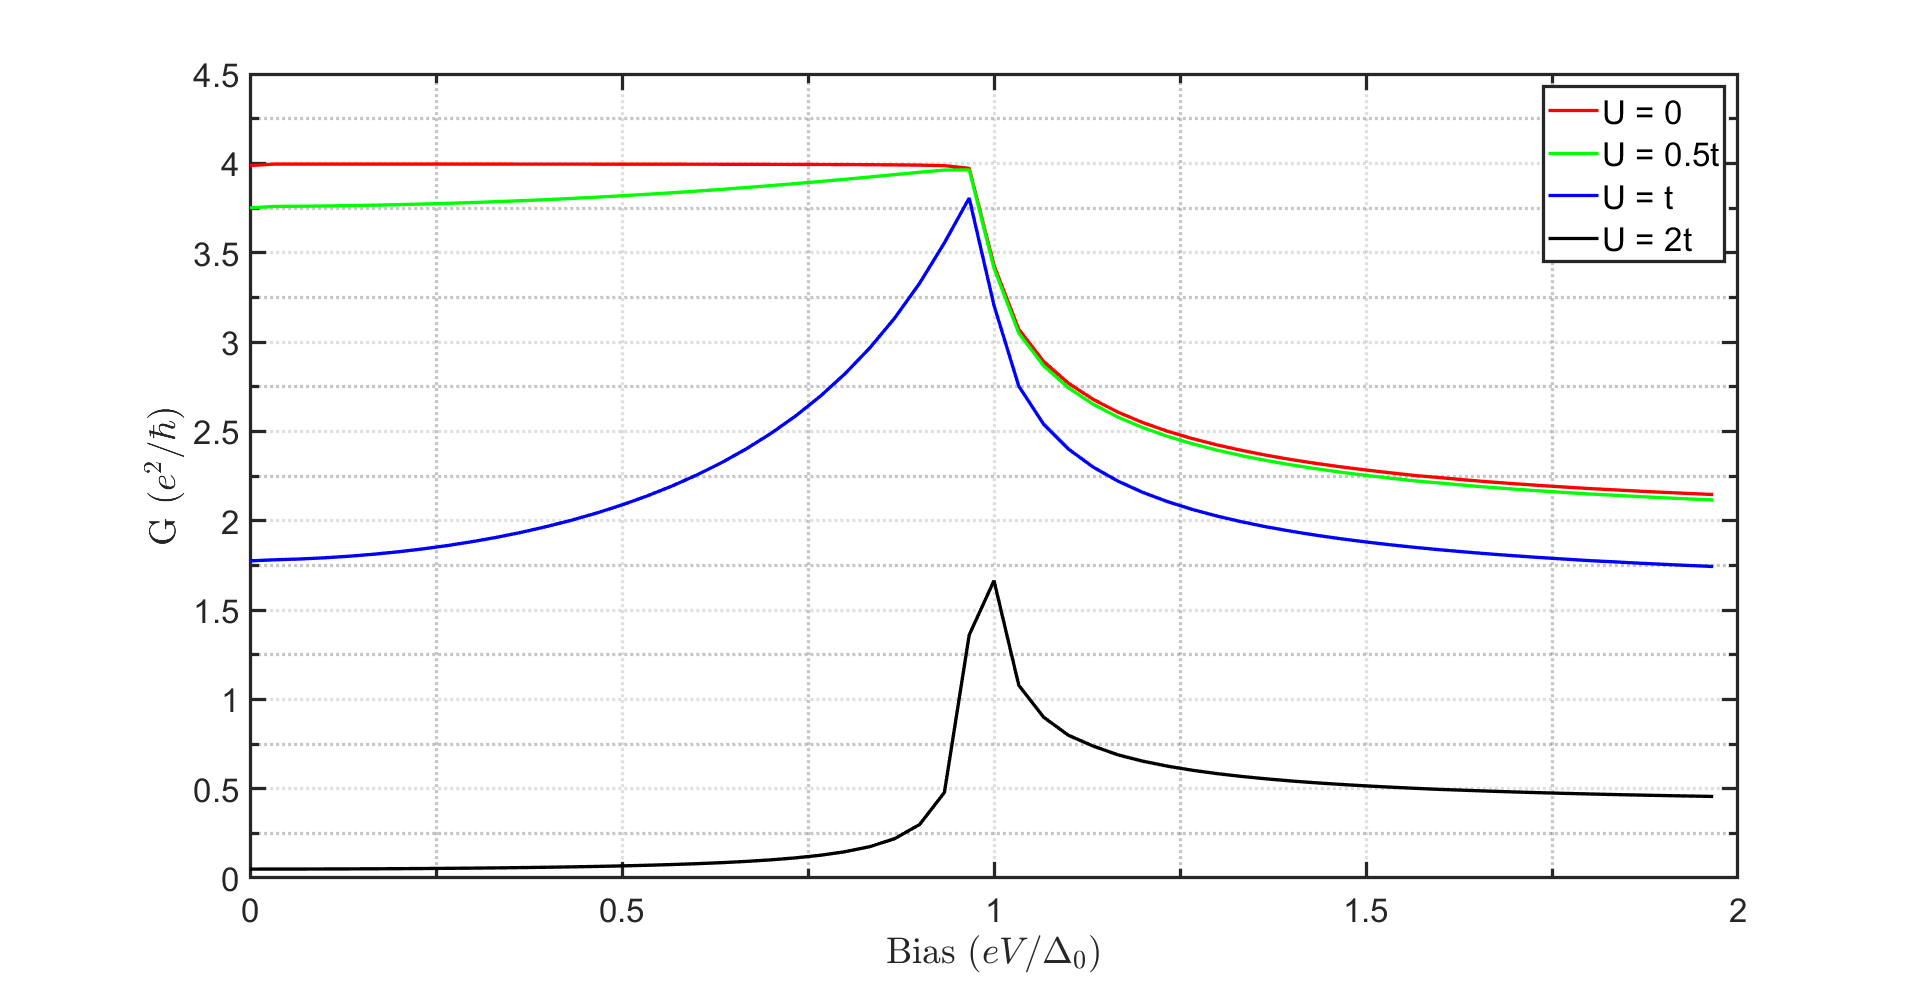
\includegraphics[scale=0.3]{G-V.png}
\caption{\textit{Conductance as a function of the applied bias across an N/S junction.}}
\end{figure}

\vspace{1cm}

A potential $U$ of varying magnitude has been introduced in the numerical simulations to simulate imperfect interfaces, which relates to the ``transparency'' of the interface. As $U$ increases, the sub-gap Andreev processes are suppressed, with increasing dominance of the direct reflection processes.


\subsection{N-S-N Structure}

In an N-S-N setup, we have two N-S interfaces, with the superconducting region acting as the device region and the two N-regions as contacts. Similar to the Fabry-Perot resonance in double barrier devices, multiple Andreev reflections give rise to resonant states termed as \textit{Andreev bound states} (ABS). The superconducting region, in particular, would be a finite Kitaev chain, which is contacted on both sides with normal leads for the remainder of this text. \par 

As discussed in \ref{subsec:NS}, the N/S junction can be visualised as two independent terminals operating at the same contact. Following from this argument, the analysis of the N-S-N setup will be based on an elaborate four-terminal device based on the Landauer-Büttiker setup. Apart from the generic direct and Andreev transmission processes, we now have an additional Andreev process termed as the crossed Andreev reflection (CAR), which corresponds to the transmission of an electrons (holes) from the left (right) contact as a hole (electron) from the right (left) contact. We can express the current across the system as a sum of three components,

\begin{equation}
    \begin{aligned}
        I^{e(h)}_{L}(E) &= \frac{e}{h}\left(\underbrace{\textbf{Tr}(\Gamma_{L}^{ee(hh)}G^{r}\Gamma_{R}^{ee(hh)}G^{a})}_{T_{D}}\:[f_{L}^{ee(hh)}(E)-f_{R}^{ee(hh)}(E)]\right)  \\
       &+ \frac{e}{h}\left(\underbrace{\textbf{Tr}(\Gamma_{L}^{ee(hh)}G^{r}\Gamma_{L}^{hh(ee)}G^{a})}_{T_{A}}\:[f_{L}^{ee(hh)}(E)-f_{L}^{hh(ee)}(E)]\right) \\
       &+ \frac{e}{h}\left(\underbrace{\textbf{Tr}(\Gamma_{L}^{ee(hh)}G^{r}\Gamma_{R}^{hh(ee)}G^{a})}_{T_{CAR}}\:[f_{L}^{ee(hh)}(E)-f_{R}^{hh(ee)}(E)]\right)
    \end{aligned}    
\end{equation}

where the third term represents the CAR process. \par 

In order to setup the transport simulations, we can potentially by-pass the tedious surface Green's function calculations by making the wide-band approximation, such that a constant density of states is assumed in the energy range of interest. This results in a constant $\gamma$ value for each relevant element of the broadening matrix $\Gamma$. \par 

Since we have two N-S interfaces, one can apply a bias across the device with a generic condition on $\mu_{L}$ and $\mu_{R}$. This can prove useful during numerical simulations, since applying a symmetric bias of $V_{L} = -V_{R} = V/2$ will nullify the crossed Andreev reflection term, $T_{CAR}$. \par 

\vspace{1cm}

\begin{figure}[h]
\centering
\includegraphics[scale=0.7]{KC_conductance.png}
\caption{\textit{Total linear conductance ($G_{A}+G_{D}$) in units of $e^{2}/h$ for $N = 20, \gamma_{L/R}/\Delta = 0.001$ as a function of $\mu/\Delta$.}}
\end{figure}

\clearpage 

\vspace*{1.5cm}

\begin{figure}[h]
\centering
\includegraphics[scale=0.65]{KC_Nsites_var.png}
\caption{\textit{Total linear conductance ($G_{A}+G_{D}$) in units of $e^{2}/h$ for $\mu = 0.0, \gamma_{L/R}/\Delta = 0.001$ as a function of $N$.}}
\end{figure}

\vspace{0.6cm}

\begin{figure}[h]
\centering
\includegraphics[scale=0.65]{KC_resonant_modes.png}
\caption{\textit{Resonant modes in the linear conductance after $t/\Delta$ exceeds a threshold value.}}
\end{figure}

\clearpage

\subsubsection{Linear Transport}

In the linear transport regime ($V \rightarrow 0, T \rightarrow 0$), the closed form expressions for the conductance of the Kitaev chain have been simulated with reference to \cite{transport_paper}. 

\vspace{0.6cm}

\begin{figure}[h]
\centering
\includegraphics[scale=0.7]{KC_GD_cmap.png}
\caption{\textit{Direct conductance term ($G_{D}$) in units of $e^{2}/h$ for $\gamma_{L/R}/\Delta = 0.001$ as a function of $\mu/\Delta$ and $t/\Delta$.}}
\end{figure}

\vspace{0.5cm}

\begin{figure}[h]
\centering
\includegraphics[scale=0.7]{KC_GA_cmap.png}
\caption{\textit{Andreev conductance term ($G_{A}$) in units of $e^{2}/h$ for $\gamma_{L/R}/\Delta = 0.001$ as a function of $\mu/\Delta$ and $t/\Delta$.}}
\end{figure}

\clearpage

\vspace*{3cm}

\begin{figure}[h]
\centering
\includegraphics[scale=1.0]{KC_Gtot_cmap.png}
\caption{\textit{Total conductance ($G_{A}+G_{D}$) in units of $e^{2}/h$ for $\gamma_{L/R}/\Delta = 0.001$ as a function of $\mu/\Delta$ and $t/\Delta$.}}
\end{figure}

\clearpage 

\subsubsection{Non-linear Transport} 

\vspace*{3cm}

\begin{figure}[h]
\centering
\includegraphics[scale=0.5]{pristine_transport_0.png}
\caption{\textit{Differential conductance of a pristine setup in units of $e^{2}/h$ as a function of $eV/2\Delta$ and $\mu/\Delta$ for $N = 21, \gamma_{L/R}/\Delta = 0.02$, and $|t/
\Delta| = 4.1$.}}
\end{figure}

\clearpage 

\vspace*{3cm}

\begin{figure}[h]
\centering
\includegraphics[scale=0.5]{disorder_transport_0.png}
\caption{\textit{Differential conductance of a disordered setup in units of $e^{2}/h$ as a function of $eV/2\Delta$ and $\mu/\Delta$ for $N = 21, \gamma_{L/R}/\Delta = 0.02$, and $|t/
\Delta| = 4.1$.}}
\end{figure}

\clearpage 

\vspace*{3cm}

\begin{figure}[h]
\centering
\includegraphics[scale=0.5]{pristine_transport_1.png}
\caption{\textit{Differential conductance of a pristine setup in units of $e^{2}/h$ as a function of $eV/2\Delta$ and $\mu/\Delta$ for $N = 21, \gamma_{L/R}/\Delta = 0.02$, and $|t/
\Delta| = 1.0$.}}
\end{figure}

\clearpage 

\vspace*{3cm}

\begin{figure}[h]
\centering
\includegraphics[scale=0.5]{disorder_transport_1.png}
\caption{\textit{Differential conductance of a disordered setup in units of $e^{2}/h$ as a function of $eV/2\Delta$ and $\mu/\Delta$ for $N = 21, \gamma_{L/R}/\Delta = 0.02$, and $|t/
\Delta| = 1.0$.}}
\end{figure}